	The overall structure of the software system contains three layers: Student Management System,
DataBase, and Queue Display System. The Student Management System is user end system which
is related to administrative functionality that includes adding, removing and editing student and staff
information in the system. The GUI allows the admin to add student and remove student. The DataBase
System is responsible for storing the information. It also allows the user to make queries. The Queue
Display System displays the information of the system and also handles the RFID listener. This is a user
end system and also includes hardware. The Queue Display System and Database System communicate
with each other to keep real time records of the student pickup.

\begin{figure}[h!]
	\centering
 	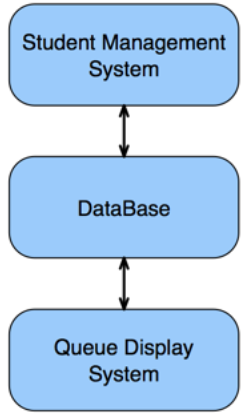
\includegraphics[width=0.40\textwidth]{./images/ads_1}
 \caption{Overall Structure of System}
\end{figure}
